
\chapter{Infraestructura}
En esta sección describiremos la infraestructura que hemos construido para el desarrollo del proyecto.
\section{Repositorio GIT}
El código del proyecto, así como las presentaciones y memoria de este proyecto, está almacenado en el 
repositorio \url{https://github.com/MaiteMartinez/MBITProject_Data4all}

\myfigure{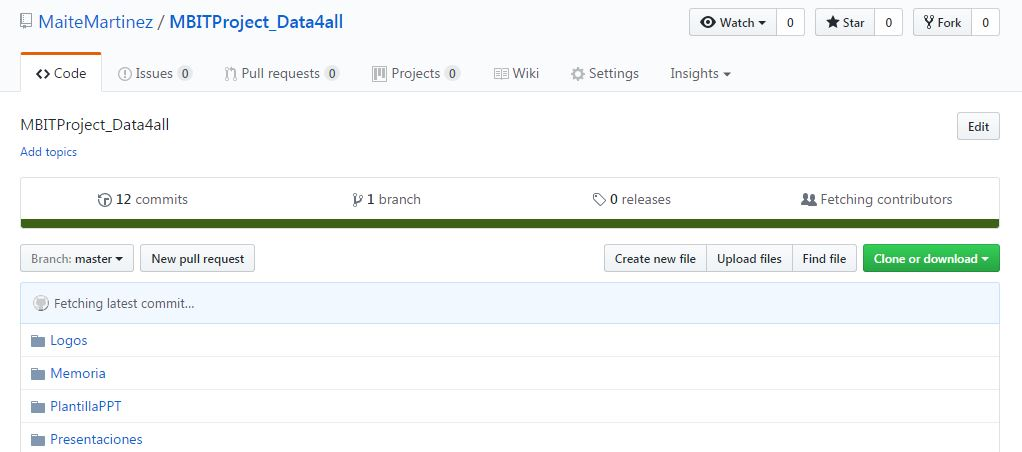
\includegraphics[width=0.6\textwidth]{repositorio_git1}%
\figcaption{Repositorio del código del proyecto.}
\label{fig:repositorio_git1} }

\section{Infraestructura para la obtención de datos}

Como muchas redes sociales, Twitter ofrece acceso a la información que generan sus usuarios a través de un
API ({\em Application Programming Interface})\cite{twitter_dev_web}. El API de Twitter ofrece diversas opciones: 
Webhook APIs, ADS API, REST APIs y Streaming APIs. La primera está enfocada a generar  
notificaciones instantáneas a partir de detección de eventos y la segunda a la integración de aplicaciones con la 
plataforma de publicidad de Twitter. Para nuestro proyecto, solo son relevantes por tanto las dos segundas:
\begin{itemize}
\item El API Rest ({\em Representational State Transfer}) permite realizar consultas puntuales con los parámetros de búsqueda indicados,
a través de una componente denominada Search API. El Search API funciona de manera similar, aunque no 
exactamente igual, a la búsqueda en la página web de Twitter. El Search API 
realiza la búsqueda entre una muestra de tuits publicados en los últimos siete días, y
las búsquedas están limitadas a 180 peticiones cada ventana temporal de 15 minutos. 

\myfigure{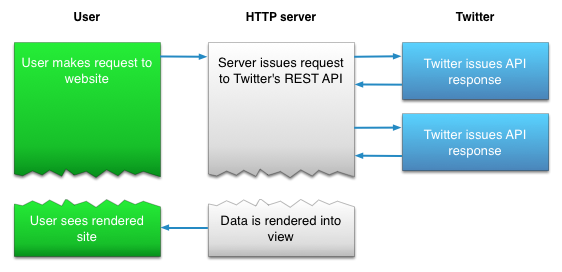
\includegraphics[width=0.6\textwidth]{api_rest_como_funciona}%
\figcaption{Funcionamiento del API Rest. \url{ https://dev.twitter.com/streaming/overview}}
\label{fig:api_rest_como_funciona} }

La búsqueda realizada por este API está centrada en la relevancia y no en la completitud, lo que 
quiere decir que algunos tuits y usuarios podrían quedarse fuera.

\item El API Streaming permite un acceso con baja latencia al flujo global de tuits de la aplicación,
y requiere una conexión HTTP continua. Entre los tipos de flujos disponibles, en la web de Twitter
para desarrolladores, se recomienda usar los flujos públicos para realizar minería de datos (en dichos flujos
aparecen muestras de los datos públicos de Twitter).

\myfigure{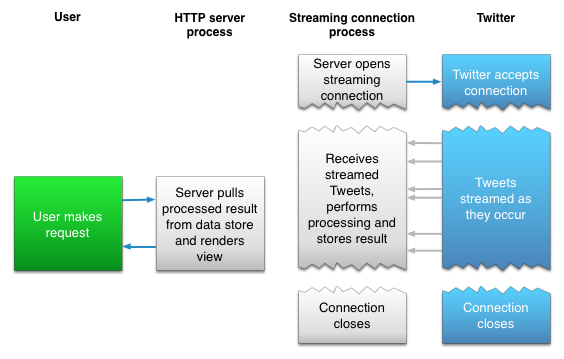
\includegraphics[width=0.6\textwidth]{api_streaming_como_funciona}%
\figcaption{Funcionamiento del API Streaming. \url{ https://dev.twitter.com/streaming/overview}}
\label{fig:api_streaming_como_funciona} }

\end{itemize}

El acceso a ambas versiones de API está gobernado por la autentificación mediante el protocolo OAuth
({\em Open Authorization}), lo que implica que para cada aplicación deben obtenerse los tokens necesarios 
de la sección de desarrolladores de Twitter, estableciéndose un número máximo de 7 por usuario.
También para ambas versiones del API existen restricciones de acceso. Estas restricciones solo
afectan a las versiones gratuitas de los APIs. Hay una versión de pago de este acceso  (Twitter Firehose)
que garantiza como respuesta el 100\% de los tuits que cumplan los criterios de la búsqueda.
Para el desarrollo de este proyecto nos hemos servido del API gratuito, por limitación de costes. 

Entre los API REST y Streaming, hemos decidido utilizar el API REST con procesos planificados de actualización frecuente 
como suficiente aproximación al tiempo real sin necesidad de usar un API Streaming que requeriría una arquitectura más compleja y robusta. 






\section{Desarrollo en la nube}